\usetikzlibrary{arrows.meta,calc}
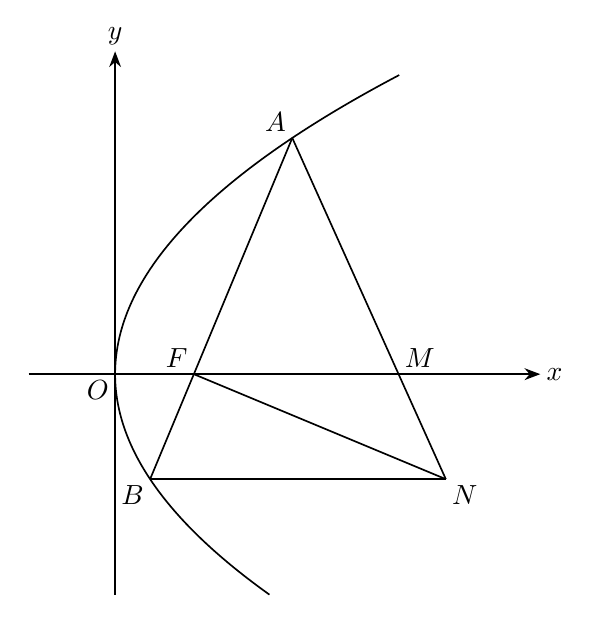
\begin{tikzpicture}[x=1cm,y=1cm,line width=.6pt,font=\normalsize,>=Stealth,
  axis/.style={line width=.6pt},
  curve/.style={line width=.6pt},
  seg/.style={line width=.6pt}]
  \coordinate (O) at (0,0);
  \coordinate (F) at (1,0);
  \coordinate (A) at (2.25,3);
  \coordinate (B) at (0.444444444,-1.333333333);
  \coordinate (M) at (3.6,0);
  \coordinate (N) at (4.2,-1.333333333);
  \draw[axis,->] (-1.1,0)--(5.4,0) node[right,inner sep=0pt,xshift=2pt] {$x$};
  \draw[axis,->] (0,-2.8)--(0,4.1) node[above,inner sep=0pt,yshift=2pt] {$y$};
  \draw[curve,domain=-2.8:3.8,samples=161] plot ({\x*\x/4},{\x});
  \draw[seg] (A)--(B);
  \draw[seg] (A)--(N);
  \draw[seg] (B)--(N);
  \draw[seg] (F)--(N);
  \node[above left,inner sep=2pt] at (A) {$A$};
  \node[below left,inner sep=2pt] at (B) {$B$};
  \node[above left,inner sep=2pt] at (F) {$F$};
  \node[above right,inner sep=2pt] at (M) {$M$};
  \node[below right,inner sep=2pt] at (N) {$N$};
  \node[below left,inner sep=2pt] at (O) {$O$};
\end{tikzpicture}
